\subsubsection{Specific colors with properties tool}\label{sec:color_properties_tool} \label{sec:colors_manually}

\begin{enumerate}
    \item Open up the Ubuntu app.
    \item Right-click on the top bar which says \textbf{Ubuntu 18.04 LTS} besides the icon logo. Press \textbf{Properties}. Go to the \textbf{Color} tab.
    \item It is a weird color tool. When pressing \textbf{Screen Text} and \textbf{Screen Background}, observe which colors that are highlighted and note it down. These must be selected just before pressing \textbf{OK} later on.
    \begin{itemize}
        \item These two selections are the main colors. The main background and main text. The selected ones, when pressing \textbf{OK} becomes the main colors.
        \item One have to be careful of changing the colors as it is hard to reset them later on.
    \end{itemize}
    \item Lets say tha you want to change this green highlight (Screen Background). Press \textbf{Screen Background} and observe which color that is highlighted and thereby is the main color. Press the same green color as the one you want to change.
    \begin{figure}[H]
        \centering
        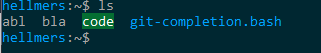
\includegraphics[width = 0.4\textwidth]{Figures/WSL/color_example.PNG}
    \end{figure}
    
    \begin{figure}[H]
        \centering
        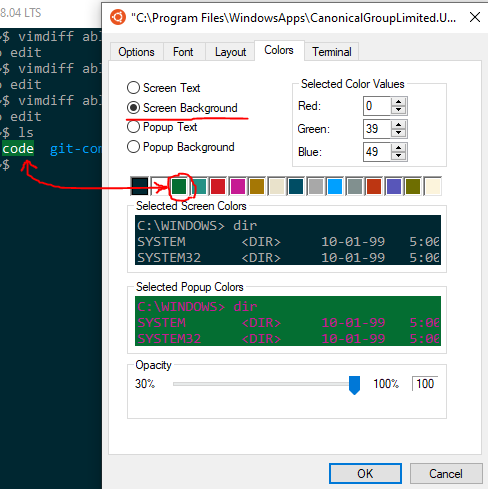
\includegraphics[width = 0.6\textwidth]{Figures/WSL/color_prompt.PNG}
    \end{figure}
    \item As the color you want to change is highlighted, change the RGB values to what you want to have instead.
    \begin{figure}[H]
        \centering
        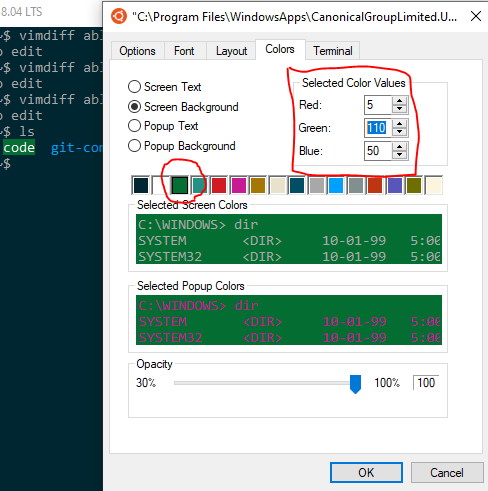
\includegraphics[width = 0.6\textwidth]{Figures/WSL/color_prompt_2.PNG}
    \end{figure}
    
    \begin{figure}[H]
        \centering
        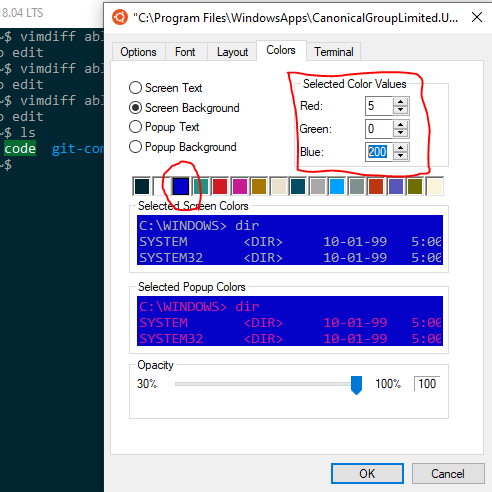
\includegraphics[width = 0.6\textwidth]{Figures/WSL/color_prompt_3.PNG}
    \end{figure}
    \item Press the previously highlighted (main color) and then press \textbf{OK}. Then the color have been changed.
    \begin{figure}[H]
        \centering
        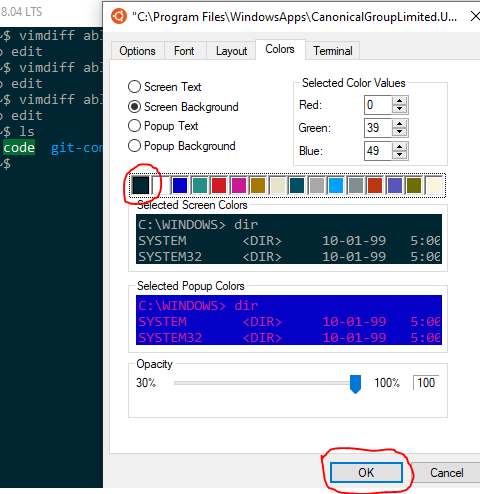
\includegraphics[width = 0.6\textwidth]{Figures/WSL/color_prompt_4.PNG}
    \end{figure}
    
    \begin{figure}[H]
        \centering
        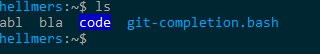
\includegraphics[width = 0.4\textwidth]{Figures/WSL/color_example_2.PNG}
    \end{figure}
\end{enumerate}

One might want to change a text color for a specific highlight color. This is done by

\begin{enumerate}
    \item Press \textbf{Screen Background}
    \item Note which color that is marked. That is the main background color.\label{item_mainbackgroundcolor}
    \item Select the highlight color which you want to change the text color for
    \item Press \textbf{Screen Text}
    \item Note which color that is marked. That is the main text color.\label{item_maintextcolor}
    \item Select the text color you want for that highlight color
    \item Press \textbf{Screen Background}
    \item Select the noted background color from step \ref{item_mainbackgroundcolor}.
    \begin{itemize}
        \item This will keep your main background color as the last selected one when pressing \textbf{OK} is the one becoming the main.
    \end{itemize}
    \item Press \textbf{Screen Text}
    \item Select the noted text color from step \ref{item_maintextcolor}.
    \begin{itemize}
        \item This will keep your main text color as the last selected one when pressing \textbf{OK} is the one becoming the main.
    \end{itemize}
\end{enumerate}
\newpage
Here are some of my colors:

\begin{figure}[H]
    \centering
    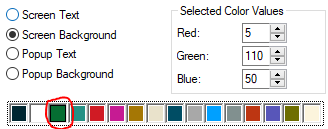
\includegraphics[width = 0.4\textwidth]{Figures/WSL/color_1.PNG}
\end{figure}

\begin{figure}[H]
    \centering
    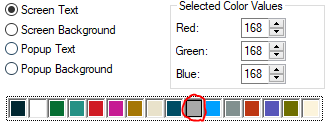
\includegraphics[width = 0.4\textwidth]{Figures/WSL/color_2.PNG}
\end{figure}

\begin{figure}[H]
    \centering
    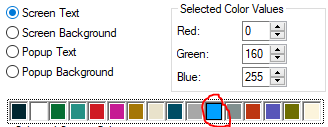
\includegraphics[width = 0.4\textwidth]{Figures/WSL/color_3.PNG}
\end{figure}